\documentclass[11pt]{article}

\usepackage[a4paper,margin=1in]{geometry}
\usepackage[T1]{fontenc}
\usepackage[utf8]{inputenc}
\usepackage{lmodern}
\usepackage{microtype}
\usepackage{amsmath,amssymb,amsthm,mathtools}
\usepackage{booktabs}
\usepackage{graphicx}
\usepackage{subcaption}
\usepackage{float}
\usepackage{enumitem}
\usepackage[numbers,sort&compress]{natbib}
\usepackage{xcolor}
\usepackage{xurl}
\usepackage[colorlinks=true,linkcolor=blue!55!black,citecolor=blue!55!black,urlcolor=blue!55!black]{hyperref}
\usepackage[nameinlink,noabbrev]{cleveref}

\setlength{\parindent}{1.4em}
\setlength{\parskip}{0.15em}
\setlist{itemsep=0.25em,topsep=0.35em}

\newtheorem{theorem}{Theorem}[section]
\newtheorem{proposition}[theorem]{Proposition}
\newtheorem{lemma}[theorem]{Lemma}
\newtheorem{corollary}[theorem]{Corollary}
\theoremstyle{definition}
\newtheorem{definition}[theorem]{Definition}
\theoremstyle{remark}
\newtheorem{remark}[theorem]{Remark}

\newcommand{\N}{\mathbb N}
\newcommand{\Z}{\mathbb Z}
\newcommand{\R}{\mathbb R}
\newcommand{\F}{\mathbb F}
\newcommand{\one}{\mathbf 1}
\newcommand{\eps}{\varepsilon}
\newcommand{\cA}{\mathcal A}
\newcommand{\cI}{\mathcal I}
\newcommand{\cP}{\mathcal P}
\newcommand{\cE}{\mathcal E}
\newcommand{\PP}{\mathbb P}
\newcommand{\Om}{\Omega}

\title{\textbf{Polynomial-Scale Rough Pairs:}\\
\textbf{Beta-Sieve Envelopes, Parity Decomposition, and a Local Bilinear Model}}
\author{Liang Wang\\
\small School of Artificial Intelligence and Automation,\\[-0.2em]
\small Huazhong University of Science and Technology, Wuhan 430074, P.R. China\\
\small \texttt{wangliang.f@gmail.com}}
\date{July 2026}

\begin{document}

\maketitle

\begin{abstract}
Let $h$ be a fixed nonzero even integer and let $S_h(X,z)$ count the integers $X<n\le2X$ for which both $n$ and $n+h$ have no prime factor below $z$.  Earlier complete-period arguments evaluate this rough-pair count only when the primorial period is negligible relative to the observation window.  We move to the polynomial cutoff $z=X^{1/u}$ and separate two further obstructions between rough pairs and prime pairs.

First, a direct application of the dimension-two Diamond--Halberstam--Richert sieve gives explicit upper and lower envelopes
\[
 S_h(X,z)=XV_h(z)\times\text{a quantity between }f_2(u)+o(1)
 \text{ and }F_2(u)+o(1).
\]
The baseline lower function is positive only beyond the DHR sifting limit $\beta_2\approx4.266$.  By contrast, if $2<u<3$, every rough survivor is exactly a prime or a semiprime.  In this latter range we unpack the first nontrivial Buchstab interval into its prime and semiprime layers and record an exact four-sector decomposition into prime--prime, prime--semiprime, semiprime--prime, and semiprime--semiprime pairs.  The prime--prime sector is a Walsh combination of three Liouville-twisted correlations and the total rough-pair count.

Second, for every fixed cutoff and fixed admissible displacement, Tao's logarithmically averaged two-point Chowla theorem implies that the four Liouville sign sectors have equal harmonic mass.  A diagonal argument preserves this conclusion along some nonquantitative, arbitrarily slow growing cutoff.  Matching harmonic and unweighted Buchstab formulas at polynomial cutoff both have a nonzero one-point parity bias, proving that even the one-point analogue of fixed-cutoff balance cannot be extended uniformly to the cubic scale.  We also diagonalize an exact complete-period bilinear roughness operator after deleting primes up to a lower cutoff: its nonconstant singular values are products of local factors $(p-2)^{-1}$.

Reproducible computations measure the four parity sectors and the factor-size distribution of semiprime contamination.  These calculations are diagnostics for possible Type~II input; they are not analytic Type~II estimates.  The paper proves no lower bound for twin primes, does not improve a prime-gap constant, and does not reduce the twin-prime problem to an independently easier assertion.
\end{abstract}

\noindent\textbf{Keywords:} beta sieve; rough numbers; prime pairs; parity problem; Liouville function; Buchstab function; bilinear operator; Type II estimate.

\medskip
\noindent\textbf{MSC 2020:} 11N35; 11N25; 11N05; 11B83; 47B15.

\section{Introduction}

For a fixed nonzero even integer $h$, the prime-pair problem asks whether there are infinitely many primes $p$ for which $p+h$ is prime.  The Hardy--Littlewood conjecture predicts the much stronger asymptotic
\begin{equation}\label{eq:hl-intro}
 \#\{X<p\le2X:p+h\in\PP\}
 \sim \mathfrak S(h)\frac{X}{(\log X)^2},
\end{equation}
where $\mathfrak S(h)$ is the pair singular series \citep{HardyLittlewood1923}.  For $h=2$, even infinitude remains open.

A finite sieve sees the local factor $\mathfrak S(h)$ exactly, but it does not distinguish a large prime from a product of large primes; this is one manifestation of the parity obstruction \citep{HeathBrown1982,FriedlanderIwaniec2010}.  In \citet{WangTwoScale2026}, complete primorial periods and centered Fourier spectra were used to separate this local information from the missing survivor-to-prime estimate.  The complete-period method yields a relative asymptotic on growing windows when the cutoff is at most logarithmic in $X$.  At the primality-exact cutoff, however, the period is exponentially larger than the window.

The present paper studies the intermediate polynomial scale
\begin{equation}\label{eq:polynomial-cutoff-intro}
 z=X^{1/u}.
\end{equation}
There are two distinct questions at this scale.

\begin{enumerate}[label=\textbf{G\arabic*.},leftmargin=3.2em]
 \item \emph{Coverage.} Can one prove that sufficiently many pairs survive all primes below $z$?
 \item \emph{Parity allocation.} If rough pairs exist, can one force any of them into the prime--prime sector rather than sectors containing semiprimes or integers with more prime factors?
\end{enumerate}

The two questions are not interchangeable.  A positive rough-pair lower bound does not force a prime pair, while an exact parity decomposition does not estimate any of its sectors.  The main purpose of this paper is to put both gaps on explicit scales.

For coverage, the sequence $n(n+h)$ has sieve dimension two.  The classical DHR beta sieve gives a positive baseline lower envelope only when the sifting parameter exceeds $\beta_2\approx4.266$ \citep{DiamondHalberstamRichert1988,DiamondHalberstam2008,Franze2011}.  Since the natural level in the present interval is $D=X^{1-o(1)}$, the parameter is $\log D/\log z=u-o(1)$.  For parity allocation, the range $2<u<3$ is especially transparent: every $z$-rough integer below $X$ has at most two prime factors.  Thus the baseline positive lower-sieve range and the exact prime/semiprime range do not overlap.

This numerical separation is a boundary of the stated DHR method, not an impossibility theorem for all analytic methods.  Results which produce primes in special sequences use additional bilinear structure, and the general framework of \citet{FordMaynard2024} shows that a substantial Type~II range is necessary for a nontrivial prime lower bound under their hypotheses.  The asymptotic sieve of \citet{FriedlanderIwaniec1998} is a central example of prime-sensitive input beyond local divisibility data.  Almost-prime correlations can also be controlled for almost all shifts in ranges where their factorization supplies a useful bilinear structure \citep{Evans2023}.  None of these results gives the fixed prime-pair asymptotic \eqref{eq:hl-intro}.

The rigorous results of this paper are as follows.

\begin{enumerate}[label=\textbf{R\arabic*.},leftmargin=3.2em]
 \item We verify the dimension-two DHR hypotheses for $n(n+h)$ with an elementary level of distribution $X/(\log X)^B$ and obtain polynomial-cutoff upper and lower envelopes.  The lower envelope becomes positive for $u>\beta_2$.
 \item For $2<u<3$, we evaluate the prime and semiprime parts of the one-dimensional rough count, both without weights and with harmonic weights.  The unweighted conditional Liouville mean converges to
 \[
  \frac{\log(u-1)-1}{1+\log(u-1)},
 \]
 so polynomial-cutoff roughness has a nonzero parity bias.
 \item In a dyadic pair window with cubic cutoff, we give an exact four-sector decomposition and Walsh inversion.  A roots-of-unity version extracts the prime sector whenever the number of possible prime factors is uniformly bounded.
 \item For fixed cutoff, logarithmically averaged two-point Chowla gives equal harmonic mass to all four Liouville sectors.  We deduce a nonquantitative slow-cutoff diagonal theorem and show why it gives no explicit polylogarithmic or polynomial range.
 \item We compute the full singular-value list of a complete-period bilinear roughness operator after deleting small primes.  This identifies deterministic local character modes but does not establish cancellation in dyadic factor boxes.
\end{enumerate}

Items R1 and R2 are standard consequences of the DHR and Buchstab frameworks, R3 is a finite Fourier identity, and R4 is a fixed-modulus consequence of \citet{Tao2016} followed by diagonalization.  We make no priority claim for these ingredients.  The contribution is their joint scale comparison, the explicit separation of coverage from factor-parity allocation, the tailored finite local model, and reproducible diagnostics.  The complete-period bilinear diagonalization is finite and exact; it does not stand in for an analytic Type~II theorem.

\subsection*{What is not claimed}

The parity projector below is an identity, not a reduction of the twin-prime problem to an easier estimate.  Proving that its prime--prime combination is $\gg X/(\log X)^2$ would already give a Hardy--Littlewood-order lower bound.  We do not infer an infinite statement from finite computations, do not transfer a complete-period mean to a polynomial cutoff, and do not infer a fixed rare event from an ordinary spectral limit.  The value $\beta_2\approx4.266$ is the sifting limit of the baseline DHR lower sieve, not a universal barrier.

\section{Polynomial rough pairs and a dimension-two beta-sieve envelope}\label{sec:dhr}

Fix a nonzero even integer $h$.  For $X>|h|$ let
\begin{equation}\label{eq:dyadic-interval}
 \cI_X=(X,2X]\cap\Z,
\end{equation}
and, for $z\ge2$, write
\begin{equation}\label{eq:rough-word}
 P(z)=\prod_{p<z}p,
 \qquad
 s_z(n)=\one_{\gcd(n,P(z))=1}.
\end{equation}
The dyadic rough-pair count is
\begin{equation}\label{eq:rough-pair-count}
 S_h(X,z)=\sum_{n\in\cI_X}s_z(n)s_z(n+h).
\end{equation}

For a prime $p$, define the local root count
\begin{equation}\label{eq:local-root-count}
 \nu_h(p)=\#\{a\bmod p:a(a+h)\equiv0\pmod p\}
 =\begin{cases}
  1,&p\mid h,\\
  2,&p\nmid h.
 \end{cases}
\end{equation}
Since $h$ is even, $\nu_h(2)=1$.  For every prime $p$ one also has the local nondegeneracy bound
\begin{equation}\label{eq:local-nondegeneracy}
 0\le\frac{\nu_h(p)}p\le\frac23<1.
\end{equation}
Extend $\nu_h$ multiplicatively to squarefree integers and put
\begin{equation}\label{eq:local-sieve-product}
 V_h(z)=\prod_{p<z}\left(1-\frac{\nu_h(p)}p\right).
\end{equation}
The corresponding singular series is
\begin{equation}\label{eq:pair-singular-series}
 \mathfrak S(h)
 =\prod_p\left(1-\frac{\nu_h(p)}p\right)
          \left(1-\frac1p\right)^{-2}.
\end{equation}
It is positive for every nonzero even $h$.

Let $F_2$ and $f_2$ denote the standard upper and lower dimension-two DHR sieve functions, normalized so that both tend to one at infinity.  Let $\beta_2$ be the sifting limit: $f_2(s)=0$ for $s\le\beta_2$ and $f_2(s)>0$ for $s>\beta_2$.  Numerical solution of the defining delay equations gives the standard tabulated value
\begin{equation}\label{eq:beta-two}
 \beta_2\approx4.266.
\end{equation}

\begin{theorem}[Polynomial-cutoff DHR envelope]\label{thm:dhr-envelope}
Fix $u>1$ and put $z=X^{1/u}$.  Then
\begin{equation}\label{eq:dhr-envelope}
 \bigl(f_2(u)+o_{h,u}(1)\bigr)X V_h(z)
 \le S_h(X,z)
 \le\bigl(F_2(u)+o_{h,u}(1)\bigr)X V_h(z).
\end{equation}
Moreover,
\begin{equation}\label{eq:vh-asymptotic}
 V_h(z)\sim
 \mathfrak S(h)\frac{e^{-2\gamma}}{(\log z)^2}.
\end{equation}
Consequently, for every fixed $u>\beta_2$,
\begin{equation}\label{eq:positive-rough-lower-bound}
 S_h(X,X^{1/u})\gg_{h,u}\frac{X}{(\log X)^2}.
\end{equation}
\end{theorem}

\begin{proof}
For a squarefree integer $d$, let
\[
 \cA_d=\{n\in\cI_X:d\mid n(n+h)\}.
\]
The Chinese remainder theorem and an endpoint count in each residue class give
\begin{equation}\label{eq:sieve-remainder}
 |\cA_d|=\frac{\nu_h(d)}dX+r_d,
 \qquad |r_d|\le\nu_h(d)\le2^{\omega(d)}.
\end{equation}
The density has dimension two because
\begin{equation}\label{eq:sieve-dimension}
 \sum_{p<t}\frac{\nu_h(p)\log p}{p}
 =2\log t+O_h(1).
\end{equation}
The finitely many primes dividing $h$ affect only the bounded term.

Take
\begin{equation}\label{eq:sieve-level}
 D=\frac{X}{(\log X)^{20}}.
\end{equation}
The elementary squarefree divisor estimate
\[
 \sum_{d<D}\mu(d)^2 14^{\omega(d)}\ll D(\log D)^{13}
\]
and \eqref{eq:sieve-remainder} give
\[
 \sum_{\substack{d<D\\d\mid P(z)}}
 \mu(d)^2 7^{\omega(d)}|r_d|
 \ll D(\log D)^{13}
 \ll \frac{X}{(\log X)^7}.
\]
This verifies the standard DHR average-remainder hypothesis with room to spare.  The sifting parameter is
\begin{equation}\label{eq:sifting-parameter}
 \frac{\log D}{\log z}=u-o(1).
\end{equation}
The dimension-two DHR fundamental theorem therefore yields \eqref{eq:dhr-envelope}; see \citet[Chapter~9, especially Theorem~9.1]{DiamondHalberstam2008} and \citet{DiamondHalberstamRichert1988}.  Continuity of the standard sieve functions permits $s=u-o(1)$ to be replaced by $u$.  The quoted value \eqref{eq:beta-two} is the DHR entry in the comparison table of \citet{Franze2011}.

Finally,
\[
 V_h(z)=
 \left[\prod_{p<z}
  \left(1-\frac{\nu_h(p)}p\right)
  \left(1-\frac1p\right)^{-2}\right]
 \prod_{p<z}\left(1-\frac1p\right)^2.
\]
The bracket tends to $\mathfrak S(h)$ and Mertens' product theorem gives \eqref{eq:vh-asymptotic}.  If $u>\beta_2$, then $f_2(u)>0$, proving \eqref{eq:positive-rough-lower-bound}.
\end{proof}

\begin{remark}[Method boundary, not impossibility]\label{rem:dhr-boundary}
For $u\le\beta_2$, the lower function in \eqref{eq:dhr-envelope} is zero, so the baseline DHR lower sieve furnishes no positive main term.  It does not say that rough pairs do not exist, nor that no refinement using bilinear or other arithmetic information can enter that range.
\end{remark}

\begin{remark}[Why this is beyond complete-period averaging]\label{rem:polynomial-beyond-period}
At $z=X^{1/u}$, the primorial satisfies $\log P(z)\sim z$, so $P(z)$ is much larger than $X$ for every fixed $u$.  Thus \cref{thm:dhr-envelope} is not a consequence of truncating complete primorial periods.  It uses residue-class information averaged through a sieve level $D=X^{1-o(1)}$.
\end{remark}

\section{The one-point Buchstab parity transition}\label{sec:buchstab}

Let $P^-(n)$ denote the least prime factor of $n>1$, and put $P^-(1)=\infty$.  Define
\begin{align}
 \Phi(X,z)&=\#\{n\le X:P^-(n)\ge z\},\label{eq:phi-rough}\\
 P_1(X,z)&=\#\{n\le X:P^-(n)\ge z,\ \Om(n)=1\},\label{eq:p1-count}\\
 P_2(X,z)&=\#\{n\le X:P^-(n)\ge z,\ \Om(n)=2\},\label{eq:p2-count}
\end{align}
where prime factors are counted with multiplicity by $\Om$.  The distinction between $P^-(n)>z$ and $P^-(n)\ge z$ affects only harmless endpoints and will not matter asymptotically.

\begin{theorem}[Parity-resolved Buchstab law]\label{thm:buchstab-parity}
Fix $2<u<3$ and set $z=X^{1/u}$.  Then every $z$-rough integer $n\le X$, other than $1$, has either one or two prime factors.  Moreover,
\begin{align}
 P_1(X,z)&\sim\frac{X}{\log X},\label{eq:p1-asymptotic}\\
 P_2(X,z)&\sim\log(u-1)\frac{X}{\log X},\label{eq:p2-asymptotic}\\
 \Phi(X,z)&\sim\bigl(1+\log(u-1)\bigr)\frac{X}{\log X},\label{eq:phi-asymptotic}\\
 \sum_{\substack{2\le n\le X\\P^-(n)\ge z}}\lambda(n)
 &\sim\bigl(\log(u-1)-1\bigr)\frac{X}{\log X}.
 \label{eq:liouville-rough-asymptotic}
\end{align}
Consequently, the conditional Liouville mean among nontrivial rough survivors satisfies
\begin{equation}\label{eq:conditional-parity-bias}
 \frac{\sum_{2\le n\le X,\,P^-(n)\ge z}\lambda(n)}
      {\#\{2\le n\le X:P^-(n)\ge z\}}
 \longrightarrow
 m(u):=\frac{\log(u-1)-1}{1+\log(u-1)}.
\end{equation}
\end{theorem}

\begin{proof}
If $\Om(n)\ge3$, then $n\ge z^3=X^{3/u}>X$, a contradiction.  Thus only the prime and semiprime layers occur.

The prime number theorem gives \eqref{eq:p1-asymptotic}, since primes below $z=o(X)$ contribute a lower-order term.  A semiprime in the rough layer can be written uniquely as $pq$ with $z\le p\le q$ and $pq\le X$.  Hence
\begin{equation}\label{eq:semiprime-sum}
 P_2(X,z)=
 \sum_{z\le p\le\sqrt X}
 \bigl(\pi(X/p)-\pi(p)+O(1)\bigr).
\end{equation}
The terms involving $\pi(p)$ and the endpoints are $O(X/(\log X)^2)$; for example,
\[
 \sum_{z\le p\le\sqrt X}\pi(p)
 \le \pi(\sqrt X)^2\ll\frac{X}{(\log X)^2}.
\]
Applying the prime number theorem uniformly for $u$ in compact subintervals of $(2,3)$, after a standard subdivision, and then setting $p=X^t$ gives
\begin{equation}\label{eq:semiprime-integral}
 P_2(X,z)
 \sim\frac{X}{\log X}
 \int_{1/u}^{1/2}\frac{dt}{t(1-t)}
 =\log(u-1)\frac{X}{\log X}.
\end{equation}
This proves \eqref{eq:p2-asymptotic}; it is also the first nontrivial interval of Buchstab's classical law \citep{Buchstab1937,MontgomeryVaughan2007}.  Summing the two layers proves \eqref{eq:phi-asymptotic}.  Finally, $\lambda=-1$ on primes and $\lambda=+1$ on semiprimes, so subtraction gives \eqref{eq:liouville-rough-asymptotic} and \eqref{eq:conditional-parity-bias}.
\end{proof}

\begin{corollary}[Prime and semiprime proportions]\label{cor:rough-proportions}
In the setting of \cref{thm:buchstab-parity},
\begin{equation}\label{eq:rough-proportions}
 \Pr(\Om=1\mid z\text{-rough})\longrightarrow
 \frac1{1+\log(u-1)},
 \qquad
 \Pr(\Om=2\mid z\text{-rough})\longrightarrow
 \frac{\log(u-1)}{1+\log(u-1)}.
\end{equation}
As $u\uparrow3$, the prime proportion tends to $(1+\log2)^{-1}\approx0.5906$, not $1/2$.
\end{corollary}

The same factor-layer transition can be measured with the harmonic weight used in logarithmic correlation theorems.  Excluding the isolated value $n=1$ is now essential because the total harmonic mass has a finite limit.

\begin{proposition}[Harmonic Buchstab parity law]\label{prop:harmonic-buchstab}
In the setting of \cref{thm:buchstab-parity}, define
\begin{align}
 H_1(X,z)&=\sum_{\substack{2\le n\le X\\P^-(n)\ge z,\ \Om(n)=1}}\frac1n,
 \label{eq:harmonic-prime-layer}\\
 H_2(X,z)&=\sum_{\substack{2\le n\le X\\P^-(n)\ge z,\ \Om(n)=2}}\frac1n.
 \label{eq:harmonic-semiprime-layer}
\end{align}
Then
\begin{equation}\label{eq:harmonic-layer-limits}
 H_1(X,z)\longrightarrow\log u,
 \qquad
 H_2(X,z)\longrightarrow
 I(u):=\int_1^{u-1}\frac{\log t}{1+t}\,dt.
\end{equation}
Consequently,
\begin{equation}\label{eq:harmonic-parity-bias}
 \frac{\displaystyle
  \sum_{\substack{2\le n\le X\\P^-(n)\ge z}}\lambda(n)/n}
 {\displaystyle
  \sum_{\substack{2\le n\le X\\P^-(n)\ge z}}1/n}
 \longrightarrow
 m_{\log}(u):=\frac{I(u)-\log u}{I(u)+\log u}<0.
\end{equation}
\end{proposition}

\begin{proof}
Mertens' theorem for reciprocal primes gives
\[
 H_1(X,z)=\sum_{z\le p\le X}\frac1p=\log u+o(1).
\]
Writing each semiprime uniquely as $pq$ with $z\le p\le q$ gives
\[
 H_2(X,z)=
 \sum_{z\le p\le\sqrt X}\frac1p
 \sum_{p\le q\le X/p}\frac1q.
\]
Uniform reciprocal-prime asymptotics on these polynomial ranges and partial summation yield
\begin{align*}
 H_2(X,z)
 &\longrightarrow
 \int_{1/u}^{1/2}
 \log\!\left(\frac{1-t}{t}\right)\frac{dt}{t}\\
 &=\int_1^{u-1}\frac{\log r}{1+r}\,dr=I(u).
\end{align*}
Prime squares have total weight $O(1/z)$ and do not affect the limit.  Since $1<t<u-1<2$ in the last integral,
\[
 0<I(u)<\int_1^{u-1}\frac{dt}{1+t}=\log(u/2)<\log u.
\]
Finally, $\lambda=-1$ on the prime layer and $\lambda=+1$ on the semiprime layer, which proves \eqref{eq:harmonic-parity-bias}.
\end{proof}

\begin{remark}[Generating polynomial]\label{rem:buchstab-polynomial}
Up to the common factor $X/\log X$, the two surviving factor layers are encoded by
\begin{equation}\label{eq:buchstab-generating-polynomial}
 Z_u(t)=t+\log(u-1)t^2.
\end{equation}
Evaluation at $t=1$ gives the total rough density, while evaluation at $t=-1$ gives the Liouville-weighted density.  This finite polynomial ceases to describe the rough set when three or more prime factors become possible.
\end{remark}

\section{Finite-factor parity decomposition}\label{sec:tomography}

We now return to pairs in the dyadic interval.  The point of this section is algebraic: once the cutoff is large enough to leave only primes and semiprimes, the prime--prime cell can be isolated exactly.  The resulting identity does not estimate that cell.

Put
\begin{equation}\label{eq:tomography-U}
 U=2X+|h|
\end{equation}
and choose a fixed exponent, with $X$ sufficiently large that
\begin{equation}\label{eq:theta-cubic-range}
 \frac13<\theta<\frac12,
 \qquad z=U^\theta,
 \qquad X-|h|\ge z.
\end{equation}
For $n\in\cI_X$, define the pair mask
\begin{equation}\label{eq:pair-mask-W}
 W_{X,z,h}(n)=s_z(n)s_z(n+h).
\end{equation}
Since $z^3>U$, every coordinate of a surviving pair is either prime or semiprime, with prime factors counted with multiplicity.  Write $P_2$ for this semiprime class and define
\begin{equation}\label{eq:walsh-moments}
 A_{ab}(X,z;h)=
 \sum_{n\in\cI_X}W_{X,z,h}(n)
 \lambda(n)^a\lambda(n+h)^b,
 \qquad a,b\in\{0,1\}.
\end{equation}
Thus $A_{00}=S_h(X,z)$.

\begin{theorem}[Exact four-sector inversion]\label{thm:four-sector-inversion}
Under \eqref{eq:theta-cubic-range}, let $N_{PP}$, $N_{P P_2}$, $N_{P_2P}$, and $N_{P_2P_2}$ denote the numbers of surviving pairs of the indicated types.  Then
\begin{align}
 N_{PP}&=\frac14(A_{00}-A_{10}-A_{01}+A_{11}),\label{eq:sector-PP}\\
 N_{P P_2}&=\frac14(A_{00}-A_{10}+A_{01}-A_{11}),\label{eq:sector-PS}\\
 N_{P_2P}&=\frac14(A_{00}+A_{10}-A_{01}-A_{11}),\label{eq:sector-SP}\\
 N_{P_2P_2}&=\frac14(A_{00}+A_{10}+A_{01}+A_{11}).\label{eq:sector-SS}
\end{align}
In particular, the survivor-to-prime remainder is exactly
\begin{equation}\label{eq:survivor-to-prime-remainder}
 A_{00}-N_{PP}=N_{P P_2}+N_{P_2P}+N_{P_2P_2}.
\end{equation}
\end{theorem}

\begin{proof}
On a surviving coordinate, $\lambda=-1$ precisely in the prime layer and $\lambda=+1$ precisely in the semiprime layer.  Hence
\[
 \one_P(n)=s_z(n)\frac{1-\lambda(n)}2,
 \qquad
 \one_{P_2}(n)=s_z(n)\frac{1+\lambda(n)}2.
\]
Multiplying the appropriate two projectors and expanding gives \eqref{eq:sector-PP}--\eqref{eq:sector-SS}.  Their sum is $A_{00}$, which gives \eqref{eq:survivor-to-prime-remainder}.
\end{proof}

The same projector can be written with the M\"obius function at a negligible algebraic cost.  Adopt the explicit convention $\mu(m)^0=1$ for every $m$, and define
\begin{equation}\label{eq:mobius-moments}
 M_{ab}(X,z;h)=
 \sum_{n\in\cI_X}W_{X,z,h}(n)
 \mu(n)^a\mu(n+h)^b.
\end{equation}
In particular, $M_{00}=A_{00}$.

\begin{corollary}[M\"obius approximation]\label{cor:mobius-projector}
For fixed $h$ in the cubic range,
\begin{equation}\label{eq:mobius-prime-projector}
 N_{PP}=
 \frac14(M_{00}-M_{10}-M_{01}+M_{11})+O_h(\sqrt X).
\end{equation}
The error is $o(X/(\log X)^2)$.
\end{corollary}

\begin{proof}
The functions $\mu$ and $\lambda$ agree on primes and on products of two distinct primes.  They differ in the present survivor set only at prime squares.  There are $O(\sqrt U)$ such values in either coordinate, so replacing all three twisted moments changes the Walsh combination by $O_h(\sqrt X)$.
\end{proof}

There is also an exact finite Fourier version when more factor layers are present.

\begin{proposition}[Roots-of-unity factor projector]\label{prop:root-unity-projector}
Let $K\ge2$, suppose $z^{K+1}>U$ and $X-|h|\ge z$, and put $\zeta=e^{2\pi i/(K+1)}$.  For every $m\in(X-|h|,U]$,
\begin{equation}\label{eq:root-unity-one-point}
 \one_{m\text{ prime}}
 =s_z(m)\frac1{K+1}
  \sum_{j=0}^{K}\zeta^{-j}\zeta^{j\Om(m)}.
\end{equation}
Consequently,
\begin{equation}\label{eq:root-unity-pair}
 N_{PP}=\frac1{(K+1)^2}
 \sum_{j,k=0}^{K}\zeta^{-j-k}
 \sum_{n\in\cI_X}W_{X,z,h}(n)
 \zeta^{j\Om(n)+k\Om(n+h)}.
\end{equation}
\end{proposition}

\begin{proof}
On the support of $s_z$, the size condition gives $1\le\Om(m)\le K$.  Orthogonality on the cyclic group $\Z/(K+1)\Z$ selects the class $\Om(m)=1$.  Applying the identity in both coordinates gives \eqref{eq:root-unity-pair}.
\end{proof}

\begin{remark}[Identity versus estimate]\label{rem:identity-versus-estimate}
For fixed $h=2$, proving that the right-hand side of \eqref{eq:sector-PP} is positive for all sufficiently large $X$ would imply the twin-prime conjecture and is strictly stronger, since it produces a prime pair in every sufficiently large dyadic interval.  The inversion exposes the cancellation that is needed, but it does not supply it.  If $z$ is only polylogarithmic, then the number $K$ of possible factor layers grows with $X$, so no fixed collection of parity twists can isolate primes exactly.
\end{remark}

\section{Fixed-cutoff logarithmic balance and a slow diagonal}\label{sec:log-balance}

The polynomial regime has a nonzero one-point parity bias in both unweighted and harmonic averages by \cref{thm:buchstab-parity,prop:harmonic-buchstab}.  At every fixed cutoff the logarithmically averaged picture is different.  The distinction is a useful warning about uniformity.

Fix a positive even $h$ and a fixed $y\ge2$.  Let
\begin{equation}\label{eq:fixed-mask}
 q=P(y),\qquad
 w_{y,h}(n)=s_y(n)s_y(n+h),
\end{equation}
and let
\begin{equation}\label{eq:fixed-mask-density}
 C_y(h)=\frac1q\sum_{r\bmod q}w_{y,h}(r)
 =\prod_{p<y}\left(1-\frac{\nu_h(p)}p\right)>0.
\end{equation}
For $a,b\in\{0,1\}$ put
\begin{equation}\label{eq:log-moments}
 L_{ab}(X;y,h)=
 \sum_{|h|<n\le X}
 \frac{w_{y,h}(n)\lambda(n)^a\lambda(n+h)^b}{n}.
\end{equation}

\begin{theorem}[Fixed-cutoff logarithmic balance]\label{thm:fixed-cutoff-balance}
For fixed $y$ and fixed positive even $h$,
\begin{align}
 L_{00}(X;y,h)&=C_y(h)\log X+O_{y,h}(1),\label{eq:L00-fixed}\\
 L_{10}(X;y,h)&=o_{y,h}(\log X),\label{eq:L10-fixed}\\
 L_{01}(X;y,h)&=o_{y,h}(\log X),\label{eq:L01-fixed}\\
 L_{11}(X;y,h)&=o_{y,h}(\log X).\label{eq:L11-fixed}
\end{align}
Equivalently, for each $\sigma,\tau\in\{-1,+1\}$,
\begin{equation}\label{eq:fixed-sign-sectors}
 \sum_{|h|<n\le X}
 \frac{w_{y,h}(n)
 \one_{\lambda(n)=\sigma}\one_{\lambda(n+h)=\tau}}n
 =\left(\frac14+o_{y,h}(1)\right)C_y(h)\log X.
\end{equation}
\end{theorem}

\begin{proof}
The untwisted mask is periodic modulo $q$, so summation over its finitely many residue classes proves \eqref{eq:L00-fixed}.  For $L_{10}$ and $L_{01}$, the prime number theorem for the Liouville function in each fixed arithmetic progression, followed by partial summation, gives the required $o(\log X)$ estimate \citep{MontgomeryVaughan2007}.  In the $L_{01}$ term, replacing $1/n$ by $1/(n+h)$ costs only $O_h(1)$.

For the double twist, choose positive representatives for the allowed residue classes $r\pmod q$ and write $n=qm+r$.  Tao's logarithmically averaged two-point Chowla theorem \citep[Theorem~1.2]{Tao2016} applies to the fixed affine forms
\[
 qm+r,\qquad qm+r+h,
\]
whose determinant is $qh\ne0$.  Replacing $(qm+r)^{-1}$ with $(qm)^{-1}$ costs $O_{q,r}(1)$.  Summing over the finite set of allowed classes proves \eqref{eq:L11-fixed}.  Expanding the two sign projectors proves \eqref{eq:fixed-sign-sectors}.
\end{proof}

For comparison, the one-point periodic mask also satisfies
\begin{equation}\label{eq:fixed-one-point-balance}
 \sum_{2\le n\le X}\frac{s_y(n)}n=V_0(y)\log X+O_y(1),
 \qquad
 \sum_{2\le n\le X}\frac{s_y(n)\lambda(n)}n=o_y(\log X),
\end{equation}
where $V_0(y)=\prod_{p<y}(1-p^{-1})$.  After normalizing by the total harmonic mass, this is the precise one-point statement whose polynomial analogue fails by \cref{prop:harmonic-buchstab}.

The fixed-cutoff theorem can be diagonalized, but the resulting growth is deliberately nonquantitative.

\begin{theorem}[Nonquantitative slow-cutoff diagonal]\label{thm:slow-diagonal}
There exist nondecreasing step functions $y(X),H(X)\to\infty$, with
\begin{equation}\label{eq:slow-cutoff-size}
 y(X)=o(\log X),
\end{equation}
such that
\begin{equation}\label{eq:slow-diagonal-twists}
 \max_{\substack{2\le h\le H(X)\\2\mid h}}
 \max_{\substack{a,b\in\{0,1\}\\(a,b)\ne(0,0)}}
 \frac{|L_{ab}(X;y(X),h)|}{C_{y(X)}(h)\log X}
 \longrightarrow0
\end{equation}
and
\begin{equation}\label{eq:slow-diagonal-mass}
 \max_{\substack{2\le h\le H(X)\\2\mid h}}
 \left|
 \frac{L_{00}(X;y(X),h)}{C_{y(X)}(h)\log X}-1
 \right|\longrightarrow0.
\end{equation}
\end{theorem}

\begin{proof}
Choose increasing sequences $y_k,H_k\to\infty$.  For fixed $k$, \cref{thm:fixed-cutoff-balance} holds simultaneously for the finite set of even $h\le H_k$.  Choose $X_k>H_k$ so large that all normalized errors are at most $1/k$ for every $X\ge X_k$, and also $y_k/\log X_k\le1/k$.  Taking $X_k$ strictly increasing and setting $y(X)=y_k$, $H(X)=H_k$ on $[X_k,X_{k+1})$ proves the claim.
\end{proof}

\begin{remark}[No quantitative transfer]\label{rem:no-uniform-chowla-transfer}
The functions in \cref{thm:slow-diagonal} are nonquantitative and may grow arbitrarily slowly after passing to a subsequence of scales.  The theorem does not permit $y=(\log X)^A$, let alone $y=X^\theta$, and it concerns harmonic rather than unweighted averages.  The nonzero harmonic limit $m_{\log}(u)$ in \eqref{eq:harmonic-parity-bias} shows that uniformity already fails for the matching one-point analogue at polynomial cutoff.  This observation does not determine the four pair sectors at polynomial scale.
\end{remark}

\section{An exact complete-period bilinear spectrum}\label{sec:bilinear-spectrum}

We next isolate a finite local operator which arises after removing small primes.  It gives an exact singular spectrum on complete residue systems.  The distinction between this calculation and an analytic Type~II estimate is essential.

Let $2\le w<y$ and suppose the set
\[
 \cP_{w,y}=\{p:w<p\le y, p\text{ prime}\}
\]
is nonempty.  Via the Chinese remainder theorem, put
\begin{equation}\label{eq:bilinear-group}
 Q_{w,y}=\prod_{p\in\cP_{w,y}}p,
 \qquad
 G_{w,y}=\prod_{p\in\cP_{w,y}}\F_p^\times.
\end{equation}
This kernel is the complete-period local model for a factor box: if an integer coordinate is written as $N=m\ell$ and $m,\ell$ are units modulo $p$, then
\begin{equation}\label{eq:factor-kernel-origin}
 p\nmid(m\ell+2)
 \quad\Longleftrightarrow\quad
 (m\bmod p)(\ell\bmod p)\ne-2.
\end{equation}
For the displacement $h=2$, define
\begin{align}
 K_{w,y}(a,b)&=
 \prod_{p\in\cP_{w,y}}\one_{a_pb_p\ne-2},\label{eq:bilinear-kernel}\\
 \kappa_{w,y}&=
 \prod_{p\in\cP_{w,y}}\frac{p-2}{p-1}.\label{eq:bilinear-kappa}
\end{align}
The corresponding centered kernel is
\begin{equation}\label{eq:centered-bilinear-kernel}
 K_{w,y}^{\circ}(a,b)=\kappa_{w,y}^{-1}K_{w,y}(a,b)-1.
\end{equation}
On $L^2(G_{w,y})$ with uniform probability measure, let
\begin{equation}\label{eq:bilinear-operator}
 (T_{w,y}f)(a)=\frac1{\kappa_{w,y}}
 \mathbb E_{b\in G_{w,y}}K_{w,y}(a,b)f(b).
\end{equation}

\begin{theorem}[Complete-period singular values]\label{thm:bilinear-singular-values}
Write a multiplicative character as $\chi=\bigotimes_{p\in\cP_{w,y}}\chi_p$.  Then
\begin{equation}\label{eq:T-character}
 T_{w,y}\chi=m(\chi)\overline\chi,
 \qquad
 |m(\chi)|=
 \prod_{\substack{p\in\cP_{w,y}\\\chi_p\ne\one}}
 \frac1{p-2}.
\end{equation}
Thus the singular-value list indexed by $\chi\in\widehat G_{w,y}$ is
\begin{equation}\label{eq:singular-value-list}
 \left\{
 \prod_{\chi_p\ne\one}(p-2)^{-1}:\chi\in\widehat G_{w,y}
 \right\}.
\end{equation}
The constant character contributes singular value $1$, and if $p_+(w,y)$ is the smallest prime in $\cP_{w,y}$, then
\begin{equation}\label{eq:mean-zero-operator-norm}
 \|T_{w,y}\|_{L^2_0\to L^2_0}
 =\frac1{p_+(w,y)-2}.
\end{equation}
\end{theorem}

\begin{proof}
It is enough to compute one local factor.  If $\chi_p$ is nontrivial, then
\[
 \sum_{\substack{b\in\F_p^\times\\ab\ne-2}}\chi_p(b)
 =-\chi_p(-2)\overline{\chi_p(a)},
\]
whereas the same sum is $p-2$ for the trivial character.  Dividing by the local normalization $(p-2)/(p-1)$ and taking the product proves \eqref{eq:T-character}.  Characters form an orthonormal basis and complex conjugation only permutes this basis, so the absolute multipliers are exactly the singular values.  On the mean-zero subspace at least one local character is nontrivial; the largest product is obtained by making only the smallest available prime nontrivial, which proves \eqref{eq:mean-zero-operator-norm}.
\end{proof}

\begin{remark}[Local obstructions and small-prime deletion]\label{rem:local-obstruction}
If $3\in\cP_{w,y}$, the mean-zero norm is $1/(3-2)=1$: a deterministic mod-$3$ character survives.  Taking $w\ge3$ and $y\ge5$ makes the first possible factor $1/(5-2)=1/3$, and sending the lower cutoff $w$ to infinity makes the complete-period mean-zero norm tend to zero.  These are exact local statements, analogous only to the local component of a $W$-trick.
\end{remark}

\begin{remark}[Not a Type II estimate]\label{rem:not-type-II}
The operator in \cref{thm:bilinear-singular-values} is averaged over a complete finite group.  It does not control a short dyadic rectangle
\begin{equation}\label{eq:type-II-box}
 \sum_{\substack{m\sim M,\ n\sim N\\(mn,Q_{w,y})=1}}
 \alpha_m\beta_n
 K_{w,y}^{\circ}(m\bmod Q_{w,y},n\bmod Q_{w,y}),
 \qquad MN\asymp X,
\end{equation}
where $|\alpha_m|,|\beta_n|\le1$.  Passing from complete residue systems to such factor boxes is the unresolved analytic transfer relevant to a Type~II argument.
\end{remark}

\section{Reproducible finite-scale diagnostics}\label{sec:numerics}

The exact projector in \cref{thm:four-sector-inversion} suggests a deterministic diagnostic.  For starts $n\in[X,2X)$, positive even $h$, and
\[
 y=\lfloor(2X+h)^\theta\rfloor,
 \qquad \frac13<\theta<\frac12,
\]
we completely factor both coordinates, impose $P^-(n),P^-(n+h)>y$, and record all four sectors and the three Liouville moments.  This strict inequality is equivalent to the continuous cutoff $P^->(2X+h)^\theta$ after taking $y$ to be its floor, except in the irrelevant case of an integral power.  For every semiprime coordinate we also record
\begin{equation}\label{eq:factor-alpha}
 \alpha=\frac{\log P^-(m)}{\log(2X+h)}.
\end{equation}
Values of $\alpha$ near $\theta$ are relatively unbalanced factorizations; values near $1/2$ are balanced.

The implementation in the accompanying \texttt{experiments/} directory is a segmented complete factor sieve in C++17.  An independent trial-division test checks all summary counts on small intervals; all factor histograms and counts are also compared across two block sizes.  The Walsh reconstruction and sector-sum errors are required to be exactly zero.  The plotting script has no nonstandard Python dependencies.  The theoretical interval $(X,2X]$ and computational interval $[X,2X)$ differ only by endpoints; every finite table uses the latter convention explicitly.

\begin{figure}[htbp]
 \centering
 \IfFileExists{figures/rough-pair-x1e8-h2.png}{%
  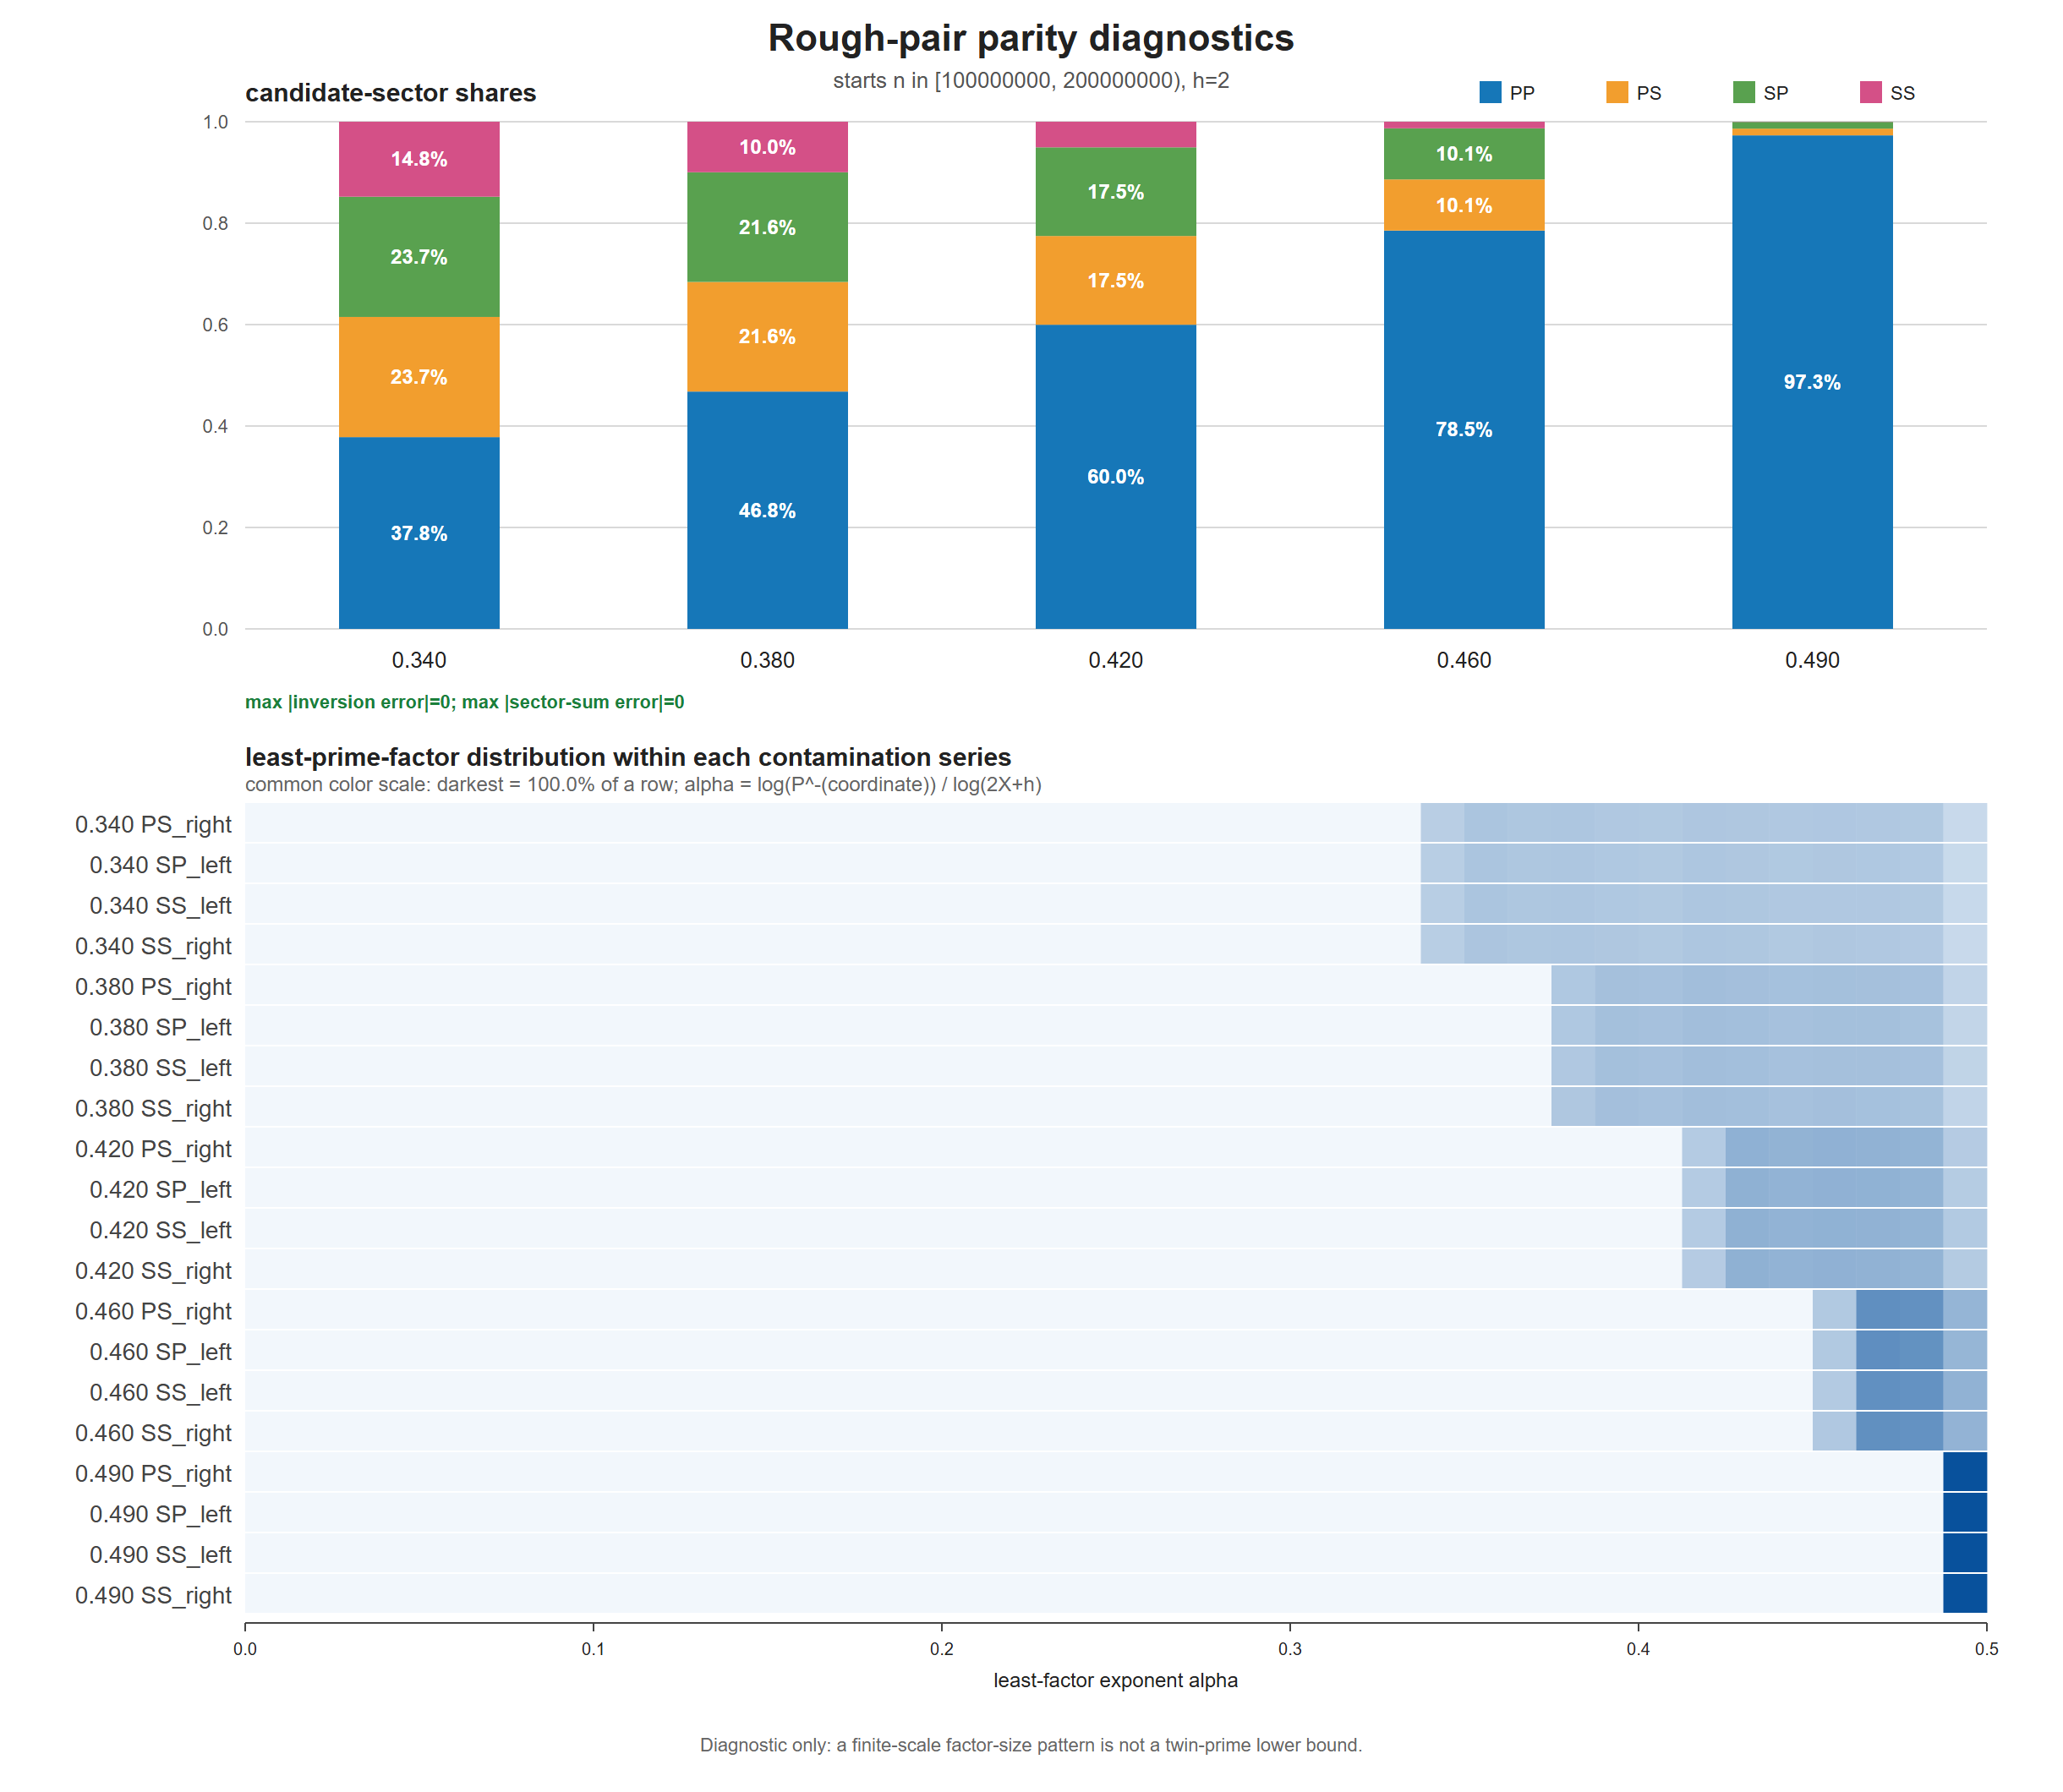
\includegraphics[width=0.98\textwidth]{figures/rough-pair-x1e8-h2.png}%
 }{%
  \fbox{\parbox[c][5.0cm][c]{0.92\textwidth}{\centering
  Reproducible diagnostic figure generated by the code in \texttt{experiments/}.}}%
 }
 \caption{Four-sector and least-factor diagnostics for $X=10^8$ and $h=2$, showing five of the nine retained cutoffs.  The top panel is an exact decomposition of the rough-pair set; the bottom panel localizes semiprime contamination by factor size on one common row-share color scale.  It is not an extrapolation to $X=\infty$.}
 \label{fig:finite-diagnostics}
\end{figure}

Three features of this computation have different logical status.  The four-sector identity is exact and tests the implementation, not a conjecture.  The movement of mass between semiprime sectors as $\theta$ changes is a finite arithmetic observation.  Any assertion of uniform cancellation in balanced factor boxes would be a new analytic estimate and cannot be inferred from the plot.

For orientation, three rows underlying \cref{fig:finite-diagnostics} are shown in \cref{tab:finite-sectors}.  The prime--prime count is independent of the cutoff throughout this range because every prime coordinate exceeds $y$; the changing total is exactly the removal of semiprime-containing pairs.

\begin{table}[htbp]
 \centering
 \caption{Exact sector counts for starts $10^8\le n<2\cdot10^8$ and $h=2$.}
 \label{tab:finite-sectors}
 \small
 \begin{tabular}{@{}rrrrrrr@{}}
  \toprule
  $\theta$ & $y$ & $A_{00}$ & $N_{PP}$ & $N_{P P_2}$ & $N_{P_2P}$ & $N_{P_2P_2}$\\
  \midrule
  $0.34$ & $664$   & $986{,}697$ & $373{,}059$ & $233{,}831$ & $233{,}910$ & $145{,}897$\\
  $0.42$ & $3{,}065$ & $622{,}068$ & $373{,}059$ & $108{,}863$ & $108{,}730$ & $31{,}416$\\
  $0.49$ & $11{,}681$ & $383{,}381$ & $373{,}059$ & $5{,}078$ & $5{,}097$ & $147$\\
  \bottomrule
 \end{tabular}
\end{table}

The retained data also contain the even shifts $h=6,10,30$ as finite controls.  They verify the same exact identities but are not used to fit a model or to infer the behavior of the prescribed shift $h=2$.

\section{A scale map and a conservative route forward}\label{sec:roadmap}

The results place four mathematically different regimes on one map:
\begin{equation}\label{eq:scale-map}
 \begin{array}{rcl}
 u>\beta_2\approx4.266
  &:& \text{positive baseline DHR rough-pair lower envelope},\\
 2<u<3
  &:& \text{exact prime/semiprime factor resolution},\\
 y\text{ fixed or nonquantitatively slow}
  &:& \text{logarithmic Liouville-sector balance},\\
 \text{complete primorial periods}
  &:& \text{exact local bilinear singular values}.
 \end{array}
\end{equation}
These statements do not presently overlap in a way that forces a prime pair.  There are two separate missing transfers.

\paragraph{Coverage transfer.}
Within the present unweighted rough-pair strategy, one possible coverage task is to move a positive lower estimate from $u>4.266$ toward a factor-resolution range such as $u<3$, or to replace it by a weighted statement that already suppresses higher factor layers.  The number $4.266$ is a baseline sieve constant, not a claim about every conceivable method.

\paragraph{Parity transfer.}
Even a positive rough-pair count with only prime and semiprime coordinates leaves four nonnegative cells.  One needs information that prevents all mass from being absorbed by the three semiprime-containing cells.  Chen's theorem illustrates how switching and bilinear estimates can force a prime plus an almost prime \citep{Chen1973,FriedlanderIwaniec2010}; it does not make the almost-prime coordinate prime.  Likewise, almost-prime correlations for almost all shifts do not provide an asymptotic for the prescribed fixed shift $h=2$ \citep{Evans2023}.

The exact spectrum in \cref{sec:bilinear-spectrum} suggests a deliberately weaker programmatic question.  Fix $\delta>0$, take $M,N\ge X^\delta$ with $MN\asymp X$, let $w=w(X)\to\infty$, and choose $y>w$ so that $Q_{w,y}$ is larger than the factor boxes and complete-period averaging is unavailable.  For coefficients $|\alpha_m|,|\beta_n|\le1$ supported on $(mn,Q_{w,y})=1$, can one prove the explicit short-box estimate
\begin{equation}\label{eq:open-bilinear-benchmark}
 \sum_{\substack{m\sim M,\ n\sim N\\(mn,Q_{w,y})=1}}
 \alpha_m\beta_n
 K_{w,y}^{\circ}(m\bmod Q_{w,y},n\bmod Q_{w,y})
 =o(MN),
\end{equation}
first for a polylogarithmic upper cutoff, or in a separately defined version averaged over even shifts?  This is a research question, not a claimed theorem.  It is intentionally weaker than a prime-pair lower bound: its role would be to quantify when the complete-period singular-value calculation survives truncation to arithmetic factor boxes.  A credible program should proceed in the order
\begin{enumerate}[label=(\roman*),leftmargin=2.5em]
 \item prove an averaged-shift or polylogarithmic-cutoff version of \eqref{eq:open-bilinear-benchmark};
 \item obtain explicit uniformity as the cutoff grows;
 \item determine whether that input improves a weighted coverage or parity estimate;
 \item only then compare the resulting theorem with the fixed shift $h=2$.
\end{enumerate}
At every stage, a theorem about average shifts, almost primes, harmonic weights, or a complete period must retain that qualifier.

\section{Conclusion}\label{sec:conclusion}

The polynomial rough-pair problem separates cleanly into coverage and parity allocation.  A dimension-two DHR sieve supplies a positive rough-pair lower envelope only in its baseline range $u>\beta_2\approx4.266$, whereas exact prime/semiprime decomposition is available for $2<u<3$.  In the latter range, one-dimensional Buchstab theory has a strict parity bias, and the pair prime cell is an exact Walsh combination whose estimation remains open.  Fixed-cutoff logarithmic Chowla cancellation survives along some nonquantitative slow diagonal but gives no polynomial-cutoff pair theorem.  Finally, the complete-period bilinear operator has an explicit local singular spectrum, while the required dyadic Type~II transfer remains absent.

This is an explicit scale comparison and diagnostic framework, not a twin-prime theorem.  Its concrete contribution is to identify which transitions are already rigorous, which are exact identities, and which analytic estimate would have to be supplied before the framework could affect a fixed prime-pair lower bound.

\section*{Data and code availability}

The C++17 implementation, dependency-free plotting script, regression test, commands, and retained finite data are included with the source repository.  All mathematical output fields are deterministic; the timing field is machine-dependent.  Source and data hashes are recorded in the experiment manifest.

\bibliographystyle{plainnat}
\bibliography{references}

\end{document}
